\section{正则化}
\subsection{概念}
过拟合(overfitting)指的是当有多个特征时,预测函数的代价可能会很低,但对于新的预测数据全都错误的情况,这会导致模型的泛化能力较差。通过进行正则化可以提高模型的\textbf{泛化能力}。

\subsection{LASSO}

以线性回归为例,以平方误差为损失函数,并将岭回归中的 L2 范数替换为 L1 范数,有
\begin{equation}
    \min_{\boldsymbol{w}}\sum\limits_{i=1}^m{(y_i - \boldsymbol{w}^\mathrm T \boldsymbol{x}_i)^2 
    + \lambda \|\boldsymbol{w}\|_1}
\end{equation}
其中正则化参数 $\lambda > 0$,上式称为 LASSO。

LASSO 易获得稀疏解,即它求得的 $\boldsymbol{w}$ 会有更少的非零分量,如下图所示:
\begin{figure}[htbp]
    \centering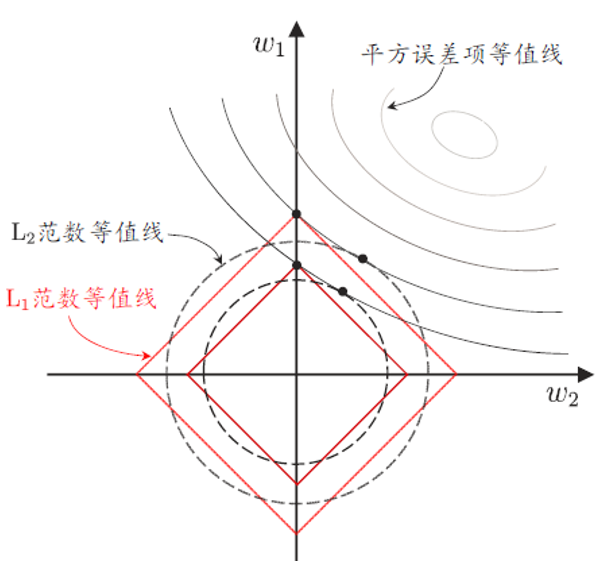
\includegraphics[scale = 0.4]{LASSO.png}
\end{figure}

可以发现,L1 范数的等值线与平方误差项的等值线的交点“常”出现在坐标轴上,即产生一个 $w_1$ 或 $w_2$ 为 0 的稀疏解,
而 L2 范数的等值线与平方误差项的等值线的交点“不太可能”出现在坐标轴上,$w_1$ 和 $w_2$ 都非 0。

\subsection{岭回归}

以线性回归为例,加入 L2 正则项后的代价函数为
\begin{equation}
    J(\boldsymbol{\theta}) = \dfrac{1}{2m}\sum_{i=1}^m(h_\theta(\boldsymbol{x}^{(i)}) - y^{(i)})^2 + \dfrac{\lambda}{2m}\sum_{\textcolor{red}{j=1}}^n\theta_j^2
\end{equation}

其中 $\lambda$ 称为正则化参数,$\lambda\sum\limits_{\textcolor{red}{j=1}}^n\theta_j^2$ 被称为 L2 正则项。

如果正则化参数过大,惩罚的程度过高,我们会得到一个除了 $\theta_0$ 以外,其他的参数都趋于零的结果,
相当于把假设函数的全部项都忽略掉了,这就导致了欠拟合的现象,欠拟合会导致\textbf{高偏差}。

如果正则化参数过小,惩罚的程度过低,相当于没有进行正则化,这就导致了过拟合的现象,过拟合会导致\textbf{高方差}。

\subsection{使用岭回归对线性回归进行正则化}
1. 梯度下降法:加入正则项后的梯度下降式为
\begin{equation}
    \begin{aligned}
        \theta_0 &:= \theta_0 - \alpha \dfrac 1m \sum\limits_{i = 1}^m {\left(h_\theta(x^{(i)}) - y^{(i)}\right)}x_0^{(i)} \\
        \theta_j &:= \theta_j - \alpha \left[\dfrac 1m \sum\limits_{i = 1}^m {\left(h_\theta(x^{(i)}) - y^{(i)}\right)}x_j^{(i)} + \dfrac{\lambda}{m}\theta_j\right]\ (j = 1, 2, 3, \dots, n) \\
        &:=\theta_{j}\left(1-\alpha \dfrac{\lambda}{m}\right)-\alpha \dfrac{1}{m} \sum_{i=1}^{m}\left(h_{\theta}\left(x^{(i)}\right)-y^{(i)}\right) x_{j}^{(i)}
    \end{aligned}
\end{equation}

2. 正规方程法:加入正则项后 $\boldsymbol{\theta}$ 的解为
\begin{equation}
    \boldsymbol\theta = \left(\mathbf{X}^{\mathrm{T}}\mathbf{X} + \lambda \begin{bmatrix}0 & & & & & \\ & 1 & & & & 
        \\ & & 1 & & & \\ & & & 1 & & \\& & & & \ddots & 
        \\ & & & & & 1\end{bmatrix}\right)^{-1}\mathbf{X}^{\mathrm{T}}y
\end{equation}

矩阵为一个主对角线上除了第一行第一列元素为 $0$,其他全为 $1$ 的 $(n + 1) \times (n + 1)$ 的矩阵。

\subsection{使用岭回归对逻辑回归进行正则化}
加入正则项后的梯度下降式为
\begin{equation}
    \begin{aligned}
        \theta_0 &:= \theta_0 - \alpha \dfrac 1m\sum\limits_{i = 1}^m\left(h_\theta\left(x^{(i)}\right) - y^{(i)}\right)x_0^{(i)} \\
        \theta_j &:= \theta_j - \alpha \left[\dfrac 1m\sum\limits_{i = 1}^m\left(h_\theta\left(x^{(i)}\right) 
        - y^{(i)}\right)x_j^{(i)} + \dfrac \lambda m \theta_j\right],\ (j = 1, 2, 3, \dots, n) \\
        &:= \left(1 - \alpha\dfrac\lambda m\right)\theta_j - \alpha \dfrac 1m\sum\limits_{i = 1}^m\left(h_\theta\left(x^{(i)}\right) 
        - y^{(i)}\right)x_j^{(i)}
    \end{aligned}
\end{equation}